\documentclass[12pt]{article}

\usepackage[letterpaper, hmargin=0.5in, vmargin=0.5in]{geometry}
\usepackage{float,graphicx,subfigure}
\usepackage{url}

\pagestyle{empty}

\title{SE465 -- Course Project}
\author{$\langle$Your Name$\rangle$ --- $\langle$Your Student ID$\rangle$ --- $\langle$Your Email$\rangle$}
\date{}

\begin{document}

\maketitle
\subsection*{(b)}

My line coverage from Jacoco is as follows.
\begin{figure}[H] %H为当前位置,!htb为忽略美学标准,htbp为浮动图形
\centering %图片居中
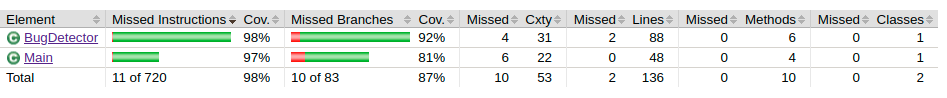
\includegraphics[width=1\textwidth]{jacoco-coverage.png} %插入图片,[]中设置图片大小,{}中是图片文件名
\end{figure}

There are several lines in BugDetector that are not covered. That is because it is a try-catch block to catch any possible I/O exceptions when reading from the provided callgraph file. Currently I do not know how to actively created such exception other than made the file unreadable by remove the read permission. However, doing that will not allow me to package that file together (because of no permission). 

In Main, although it shows that it's not 100\% covered, the report did not show any line that is not covered. In fact, when I go to the pit-test report, it says that I've reached 100\% line coverage for my Main class. Therefore, I will assume that is some brackets lines or some other lines that are not actual codes. As a support, here is the report from pit-test:

\begin{figure}[H] %H为当前位置,!htb为忽略美学标准,htbp为浮动图形
\centering %图片居中
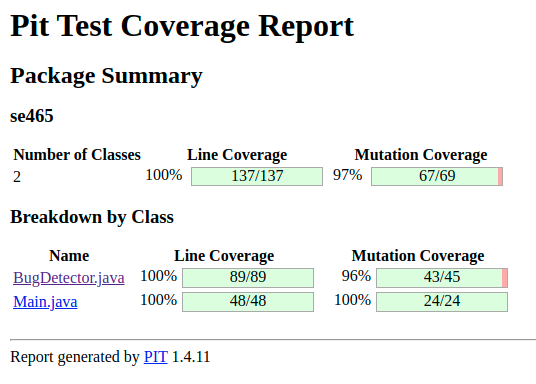
\includegraphics[width=0.7\textwidth]{pittest-coverage.png} %插入图片,[]中设置图片大小,{}中是图片文件名
\end{figure}

\newpage
\subsection*{(c)}

Generally speaking, I did not get much bugs when I use these two tools. 

From pmd, I got:
\begin{itemize}
	\item Useless paranhesis on (\&\&)
	\item Unused import -- Path. Hashset
\end{itemize}

From spotbugs, I got:
\begin{itemize}
	\item DM\_DEFAULT\_ENCODING
	\item ICAST\_IDIV\_CAST\_TO\_DOUBLE
	\item OS\_OPEN\_STREAM
	\item VA\_FORMAT\_STRING\_USES\_NEWLINE
\end{itemize}

And all of them are real bugs or code smells, although they are pretty tiny issues. For pmd ones, I simply removed those unused imports, and re-write my logic expression in one if statement. I would doubt the useless parentheses one, since in my own opinion, those parentheses will help code readers to understand the logic expression better and quicker. Maybe pmd should be more loose about parentheses checks.

For spotbugs ones, I added default encoding UTF-8 in each read and write stream, casted integer to floating numbers before doing division, added close clause to close file streams, and change new-line character slash n (\\n) to percent n (\%n). I would say these reports are pretty useful. For example, the ICAST\_IDIV\_CAST\_TO\_DOUBLE is a but that is easy to be ignored. Our support numbers are all integers, but we are doing a division to get a percentage, which means I will get a huge difference if I directly divide these two numbers which will results in an integer division. And since it is an error that is so tiny that I might will need to spend hours to figure that out. So this tool indeed helped me a lot. However, there are some reports that I do not really understand if it will have an extra effect. The VA\_FORMAT\_STRING\_USES\_NEWLINE one, according to their official documentation, they said that ``it is generally preferable better to use \%n, which will produce the platform-specific line separator.''. I will say it is very good to know this, but to be honest I do not know if this is generally true. 

One last thing I want to mention is that spotbugs have a very good code documentation that I can quickly figure out the exact bug and relavent explanation from the error code. 

\subsection*{(e)}

Here is my report for mutation coverage:
\begin{figure}[H] %H为当前位置,!htb为忽略美学标准,htbp为浮动图形
\centering %图片居中
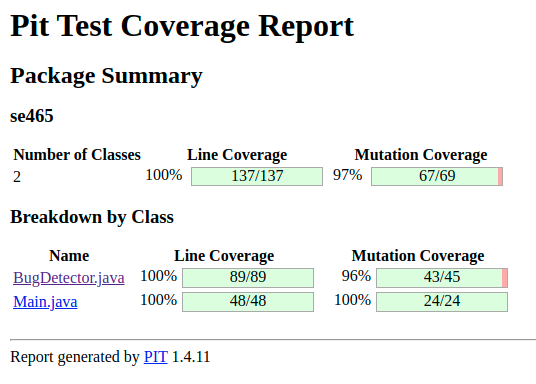
\includegraphics[width=0.7\textwidth]{pittest-coverage.png} %插入图片,[]中设置图片大小,{}中是图片文件名
\end{figure}

Specifically, I failed two for my BugDetector class. The first one is ``deleting the code'':

\begin{figure}[H] %H为当前位置,!htb为忽略美学标准,htbp为浮动图形
\centering %图片居中
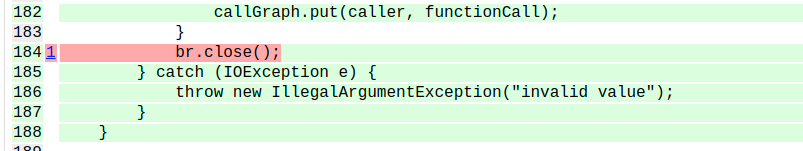
\includegraphics[width=1\textwidth]{mutation1.png} %插入图片,[]中设置图片大小,{}中是图片文件名
\end{figure}

Unfortunately I cannot find one way to test this case because this is a read stream. Even if we do not close the stream, there will be no change to the input file, and there is not any way to test it (tried Google but no good result). In fact, in some cases Java garbage collector will also close the stream (not guaranteed though). That's why I believe this line is not testable.

The second mutation test is this:
\begin{figure}[H] %H为当前位置,!htb为忽略美学标准,htbp为浮动图形
\centering %图片居中
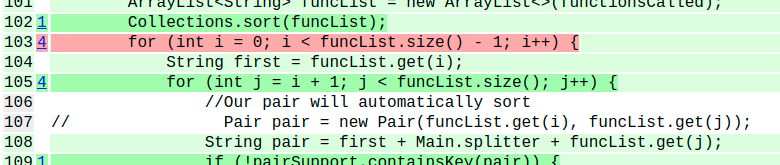
\includegraphics[width=1\textwidth]{mutation2.png} %插入图片,[]中设置图片大小,{}中是图片文件名
\end{figure}

The mutation is to make the boundary <=. I believe my programm will have the exact same behaviour in this case. Before the mutation, my outer loop will reach index size-2, and the last pair will be (size-2, size-1). After the mutation, my i will be size-1. However, my j will be size, which is out of index boundary, thus the inner loop is not running, so we still end up doing nothing. In other words, this is a equivalent mutant. However, I believe if the mutation changes two boundaries at the same time (i.e, both becomes <=), then it will be a different behaviour, and my test will kill that mutation. 



\end{document}
